%% LaTeX Beamer presentation template (requires beamer package)
%% see http://bitbucket.org/rivanvx/beamer/wiki/Home
%% idea contributed by H. Turgut Uyar
%% template based on a template by Till Tantau
%% this template is still evolving - it might differ in future releases!

\documentclass[10pt]{beamer}

\mode<presentation>
{
\usetheme{Malmoe}

\setbeamercovered{transparent}
}


\addtobeamertemplate{navigation symbols}{}{%
\usebeamerfont{footline}%
\usebeamercolor[fg]{footline}%
\hspace{1em}%
\insertframenumber/\inserttotalframenumber
}

\useoutertheme{infolines}
\setbeamertemplate{footline}{} 

\usepackage[brazil]{babel}
\usepackage[utf8]{inputenc}
\usepackage{listings}

% font definitions, try \usepackage{ae} instead of the following
% three lines if you don't like this look
\usepackage{mathptmx}
\usepackage[scaled=.90]{helvet}
\usepackage{courier}
\usepackage{url}


\usepackage[T1]{fontenc}

\title{Extensão de um elemento do artigo \textit{Accelerating Decoupled
Look-ahead via Weak Dependence Removal: A Metaheuristic Approach}}

%\subtitle{}

% - Use the \inst{?} command only if the authors have different
%   affiliation.
%\author{F.~Author\inst{1} \and S.~Another\inst{2}}
\author{Gustavo Ciotto Pinton}

% - Use the \inst command only if there are several affiliations.
% - Keep it simple, no one is interested in your street address.
\institute
{

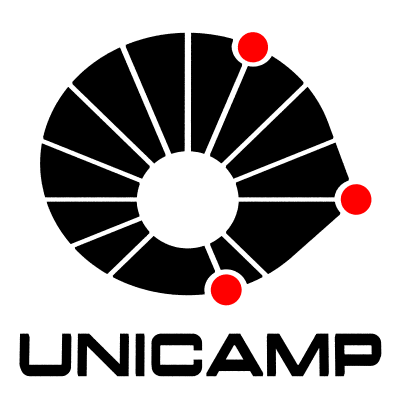
\includegraphics[scale=0.12]{logo} \\
\vspace{16pt}
Universidade Estadual de Campinas - UNICAMP\\
MO601B - Arquitetura de Computadores}

\date{18 de Novembro de 2016}



% If you have a file called "university-logo-filename.xxx", where xxx
% is a graphic format that can be processed by latex or pdflatex,
% resp., then you can add a logo as follows:

% \pgfdeclareimage[height=0.5cm]{university-logo}{university-logo-filename}
% \logo{\pgfuseimage{university-logo}}



% Delete this, if you do not want the table of contents to pop up at
% the beginning of each subsection:
\AtBeginSubsection[]
{
\begin{frame}<beamer>
\frametitle{Outline}
\tableofcontents[currentsection,currentsubsection]
\end{frame}
}

% If you wish to uncover everything in a step-wise fashion, uncomment
% the following command:

%\beamerdefaultoverlayspecification{<+->}

\begin{document}

\begin{frame}

\titlepage
\end{frame}

\begin{frame}
\frametitle{Sumário}
\tableofcontents
\end{frame}


\section{Arquitetura Decoupled Look-Ahead}

\begin{frame}
\frametitle{Arquitetura \textit{Decoupled Look-Ahead}}
\framesubtitle{Relembrando\ldots}

\begin{itemize}
\item \textit{Parser} que transforma o binário do programa principal em uma
versão reduzida, somente para procurar \textit{misses}.
\item Versão esqueleto roda em \textit{core} separado, anteriormente ao programa
principal.
\item Os resultados de saltos condicionais são transmitidos através
de uma fila para o \textit{core}.
\end{itemize}

\centering
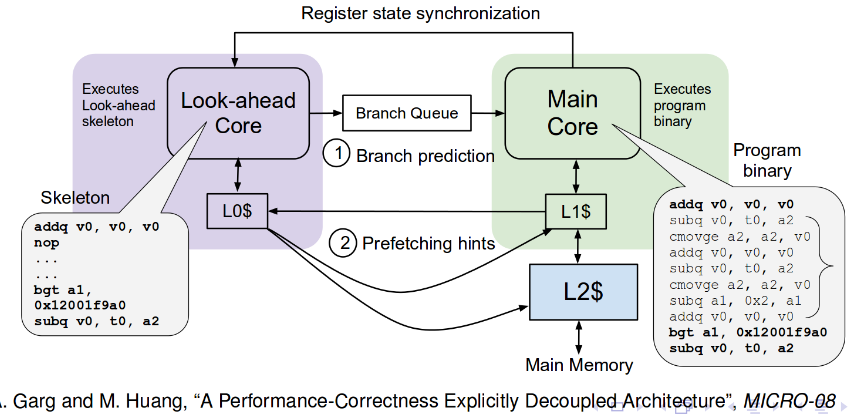
\includegraphics[width=0.9\textwidth]{images/look-ahead}

\end{frame}

\begin{frame}
\frametitle{Proposta do artigo}
\framesubtitle{Relembrando\ldots}

\begin{itemize}
\item Constatou-se que a \textit{thread} auxiliar, isto é, a \textit{look ahead
thread} se tornou o novo limite de velocidade do sistema.

\vspace{12pt}

\item A corretude da \textit{look-ahead thread} não é exigida, permitindo várias
otimizações

\begin{itemize} 
	\item Dependências fracas: instruções que contribuem marginalmente para o
	resultado e, portanto, podem ser retiradas.
	
\end{itemize} 

\vspace{12pt}

\item O artigo propõe uma
maneira de otimizá-la a partir de algoritmos genéticos:
 
\begin{itemize} 
	\item Identificação dos pontos desnecessários que poderiam ser retirados desta
	\textit{thread}. 
  
  	\item Caracterização de genes e cromossomos. 
	
\end{itemize} 
\end{itemize}

\end{frame}

\section{Projeto 3}

\begin {frame}
\frametitle{Projeto 3}
\framesubtitle{Relembrando\ldots}
\begin{itemize}
\item Reprodução das curvas \textit{ideal} e \textit{single-thread} da figura 3.
\end{itemize}

\vspace{16pt}
\centering
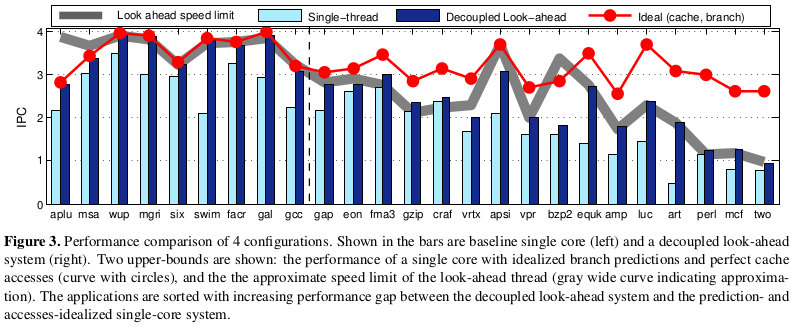
\includegraphics[width=1\textwidth]{images/fig3} 
\end{frame}

\begin{frame}
\frametitle{Projeto 3}
\framesubtitle{Resultados - \textit{Gainestown}}

\centering
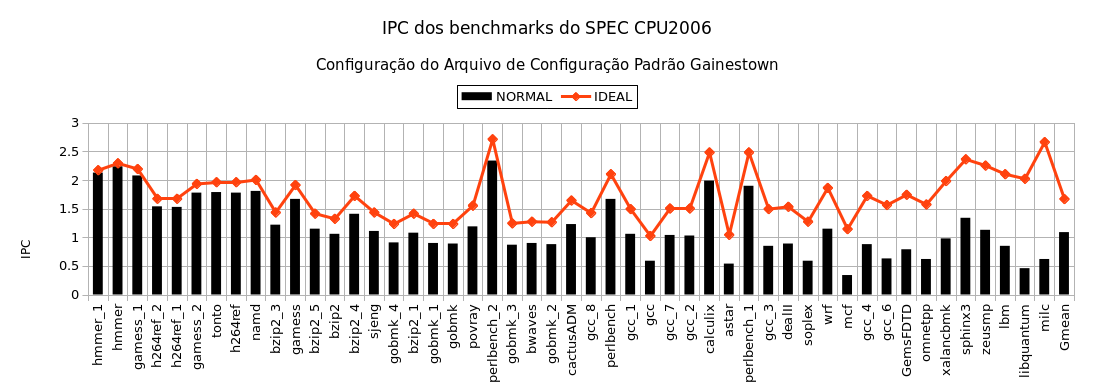
\includegraphics[width=0.87\textwidth]{images/gainestown}

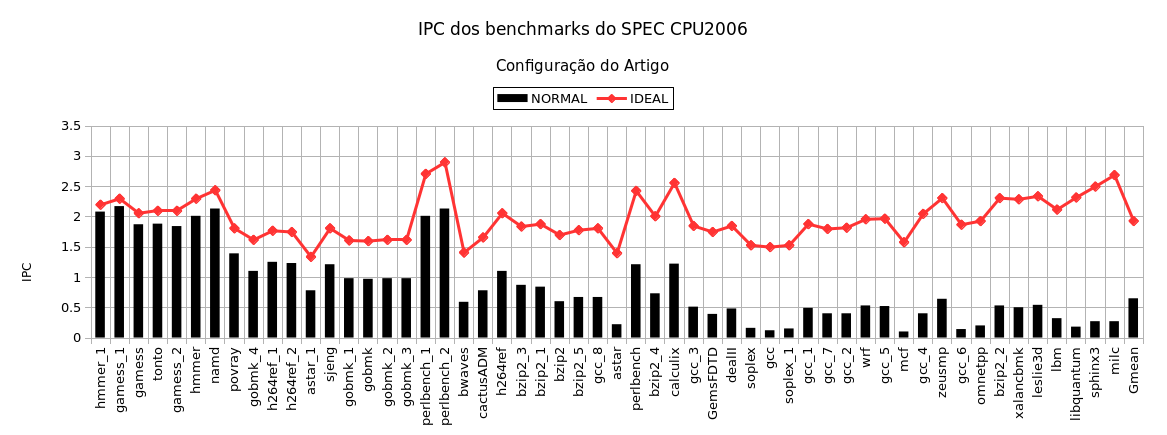
\includegraphics[width=0.87\textwidth]{images/article}

\end{frame}

\section{Projeto 4}

\begin{frame}
\frametitle{Projeto 4}
\framesubtitle{Introdução}

\begin{itemize}

\item Parâmetro modificado: tamanho das páginas de memória:

\begin{itemize} 
	\item 4KB e 4MB.
	\item Projeto 2: número de acessos adicionais à memória. 
	\item Projeto 4: efeitos da alteração no IPC.
		
\end{itemize} 

\vspace{12pt}

\item Modificações em relação ao projeto 3:
 
\begin{itemize} 
	\item \textit{Pinballs} com 100M \textit{warmup} e 30M região detalhada:
	recálculo de todos os resultados anteriores.
  
  	\item Problema com a propriedade \path{perf_model/dram/latency}:
  	\textit{sniper} a interpreta como nanossegundos e não como ciclos.
	
\end{itemize} 
\end{itemize}

\end{frame}

\begin{frame}
\frametitle{Projeto 4}
\framesubtitle{Implementação}

\begin{itemize}

\item Classe TLB do \textit{sniper} modificada:

\begin{itemize} 
	\item 3 constantes importantes: \texttt{SIM\_PAGE\_SHIFT},
	\texttt{SIM\_PAGE\_SIZE} e \texttt{SIM\_PAGE\_MASK}.
	\item \texttt{SIM\_PAGE\_SIZE} = (1 << \texttt{SIM\_PAGE\_SHIFT})
	\item \texttt{SIM\_PAGE\_MASK} = \(\sim\) (\texttt{SIM\_PAGE\_SHIFT} - 1)
	\item Por padrão: \texttt{SIM\_PAGE\_SHIFT} = 12 (4KB)
	\item Alterações no construtor da classe. 
		
\end{itemize} 

\item Criação de uma nova opção \path{perf_model/tlb/page_size_bits}:
 
\begin{itemize} 
	\item Classe \texttt{MemoryManager} lê essa propriedade e instancia TLBs.
\end{itemize}

\item Estrutura das \textit{caches}:

\begin{itemize}
  	\item 2 níveis.  
	\item I-TLB: 128 entradas e \textit{4-way associative}.
	\item D-TLB: 64 entradas e \textit{4-way associative}.
	\item STLB: TLB compartilhada com 512 entradas e \textit{4-way associative}.
\end{itemize}
 
\end{itemize}

\end{frame}

\begin{frame}
\frametitle{Projeto 4}
\framesubtitle{Resultados}


\end{frame}

\section{Referências}
\begin{frame}
\frametitle{Referências}

\begin{itemize}
  \item Carison, T. E. (2012). Interval simulation.
  \url{http://snipersim.org/w/Interval_ Simulation}. 
\item Carison, T. E. and Heirman, W. (2013). The Sniper User Manual.
\item Parihar, R. and Huang, M. C. (2014). Accelerating decoupled look-ahead via
weak dependence removal: A metaheuristic approach. International Symposium on High Performance Computer Architecture.
\end{itemize}

\end{frame}



\end{document}
